\chapter{Framework and Strategies Evaluation}
\label{chap:strategies}

\subsection{Tests}
\tab{fig:recapTests} summarizes which tests have been run.
All of them have the same terminating condition, which is reached when at least one
node finds a safety oracle at height 4. The number of nodes is chosen at random
in the interval \([1, 20[\). It has been decided to perform tests on this
interval because it is large enough to give an insight on the behavior of the
relations between the metrics, and small enough to reach the terminating condition in
a reasonable time (1 run with a number of nodes chosen at random takes on average 1 hour
with the Maximal overhead strategy).

\todo{renove table}

\begin{table}[H]
    \centering{
        \begin{tabular}{|c|c|c|}
            \hline
            & All receivers & Some receivers \\
            \hline
            Round-robin & \checkmark & \checkmark\\
            \hline
            Double round-robin & \checkmark & \checkmark\\
            \hline
            Maximal overhead & (\checkmark) & (\checkmark) \\
            \hline
            Arbitrary & \checkmark & \checkmark\\
            \hline
        \end{tabular}
        \captionsetup{justification=centering}
        \caption{Summary of tests that have been run. A tick in parenthesis
        implies that tests were run but that there are not many data points or
        big disparities in the distribution of the number of nodes}
        \label{fig:recapTests}
    }
\end{table}

\todo{schema with what to measure}
\todo{how the measurements take place in the code}

\section{Visualization I: All receivers}
This chapter presents a visualization of the data obtained through the multiple
test runs with the All receivers strategy.  Each subsection shows the results
using 3 histograms, representing the raw data, followed by 3 scatter plots
picturing each metric against each other. These graphs also show a simple linear
regression as an attempt to find a relation between each metric. At the end of
the discussion of each strategy a linear regression is performed in order to
find the scores of each variable according to the model presented in
\ssec{ssec:model}.


\todo{3D plotting?}
\todo{undersampling issue?}

\subsection{Round-robin}

\FloatBarrier

The distributions of the number of nodes and the latency
(\fig{fig:distRR} left and center) have the same
shapes except for the gaps every 3 steps. The resemblance in shape is explained
by the fact that the latency is strictly correlated to the number of nodes, as
expected.
The gaps will be explained at the end of the section, using the graphs that show
relations between variables.

\triplefigure
    {hist_nb_nodes_rr_20_nodes_4_depth_all_receivers_gen_averages}
    {hist_latency_rr_20_nodes_4_depth_all_receivers_gen_averages}
    {hist_overhead_rr_20_nodes_4_depth_all_receivers_gen_averages}
    {Distributions of the dataset for the round-robin strategy and all
    receivers. As the latency (top-right) presents a linear correlation with the number of
    nodes (top-left), the shapes of the histograms are similar. The overhead
    (bottom) always
    equals to 1 because only one message is sent per step, and each step
    finalizes a block.}
    {fig:distRR}

The histogram for the overhead is easy to analyse as well; the overhead is
expected to be 1 because once consensus is obtained for the genesis block, only
one message from the next validator is needed to finalize the next block.

\triplefigure
    {relation_nb_nodes_latency_rr_20_nodes_4_depth_all_receivers_gen_averages}
    {relation_nb_nodes_overhead_rr_20_nodes_4_depth_all_receivers_gen_averages}
    {relation_overhead_latency_rr_20_nodes_4_depth_all_receivers_gen_averages}
    {The round-robin strategy shows a linear relation between the number of
    nodes and the latency (top-left). The overhead is a constant for this
    strategy (top-right, bottom).}
    {fig:relRR}

The right and center graphs on \fig{fig:relRR} do not give more insight on the
data, as the Overhead is always \(1\). On the other hand, the graph on the left
shows a clear linear relationship between the latency and the number of nodes.
The fitted line has the following equation:
\[l = 1.403402\cdot n\]
The latency is expected to be around \(1.5\cdot n\) because the finality is
reached when at least 50\% of the network has acknowledged that the whole
network has the finalized message in its justification. As pictured in the
top-left graph of \fig{fig:relRR}, the fitted line has a slightly small
slope compared to the data points due to the fact that the line is fitted to be
linear and the data points are close the origin. \todo{insert line with 1.5*n
?}\
The gaps in the histogram showed in \fig{fig:distRR} are explained by the fact
that we expect the relation to be \(l = 1.5\cdot n\), and therefore the span of
the latency distribution is bigger than the one for the number of nodes. The
regularity of the gaps (which appear to be every 3 units of latency), is caused
by the regularity of the sending and receiving strategies. As all nodes receive
the messages at the same time, they all finalize the same blocks together, and
there cannot be a non-integer average value for the latency in this case.

\FloatBarrier
\subsection{Double round-robin}
\triplefigure
    {hist_nb_nodes_double_rr_20_nodes_4_depth_all_receivers_gen_averages}
    {hist_latency_double_rr_20_nodes_4_depth_all_receivers_gen_averages}
    {hist_overhead_double_rr_20_nodes_4_depth_all_receivers_gen_averages}
    {Distributions of the dataset for the double round-robin strategy and all
    receivers. As the latency (top-right) and the number of nodes (top-left) are
    linearly correlated, their distributions are of similar shapes. The
    overhead (bottom) equals 2, as expected and shows an outlying value at 4.}
    {fig:distDRR}

As for the simple round-robin case, the latency and number of nodes
distributions show a similar shape. The latency is less spread than for the
singl round-robin, which explains some dissimilarities between the
distributions. The distribution of the overhead presents a peak at 2, which is
expected but also shows that there are some messages that have double this
overhead, at 4. This will be explained using the following graphs. \todo{explain
outliers}

\triplefigure
    {relation_nb_nodes_latency_double_rr_20_nodes_4_depth_all_receivers_gen_averages}
    {relation_nb_nodes_overhead_double_rr_20_nodes_4_depth_all_receivers_gen_averages}
    {relation_overhead_latency_double_rr_20_nodes_4_depth_all_receivers_gen_averages}
    {The double round-robin strategy shows a linear relation between the number of
    nodes and the latency (top-left). The overhead is a constant for this
    strategy (top-right, bottom). The top-right plot indicates that the outliers
    only emerge when the tests are run with 3 or 5 nodes.}
    {fig:relDRR}

As for the simple round-robin strategy, the plots including the Overhead are not
of much use here, except they show that its value is 2, as it is expected. 
On the other hand, the plot on the top-left of \fig{fig:relDRR} shows a
linear relation between the number of nodes and the latency: 
\[l = 0.721750 \cdot n\]
This value is about half of the slope obtained for the same relation with the
round-robin strategy. The double round-robin strategy was supposed to show half
the latency with respect to the simple round-robin and this value is therefore
correct. The value of 2 for the overhead is also twice the overhead for the
single round-robin and confirms the hypothesis.
    

\FloatBarrier
\subsection{Triple round-robin}
The triple round-robin strategy shows  the same kind of information as the
double round-robin one. The overhead is 3 for almost all cases (this will be
discussed later), and the number of nodes and latency are linearly correlated.
\triplefigure
    {hist_nb_nodes_triple_rr_20_nodes_4_depth_all_receivers_gen_averages}
    {hist_latency_triple_rr_20_nodes_4_depth_all_receivers_gen_averages}
    {hist_overhead_triple_rr_20_nodes_4_depth_all_receivers_gen_averages}
    {Distributions of the dataset for the triple round-robin strategy and all
    receivers. As the latency (top-right) and the number of nodes (top-left) are
    linearly correlated, their distributions are of similar shapes. The
    overhead (bottom) equals 3, as expected and shows two outlying values at 1
    and 6.}
    {fig:distTRR}

The relationship with the overhead are again not of much use because its value
is always 3. Again, there is a linear relationship between the latency and the
number of nodes, which follows this equation:
    \[l = 0.496152 * n\]
The slope is a third as the slope for the simple round-robin strategy. Moreover
the overhead is three times larger for the triple round-robin than it is for the
simple.
\fig{fig:relTRR} shows clear outliersfor the overhead value when running
2, 5 and 11 nodes. When running 2 nodes, which is an obvious edge case for this
strategy (as there are only 2 nodes and there should be at least 3 to send
different messages), the overhead is only 1 because only one node sends a
message in this case. 

\todo{explain other outliers}
\triplefigure
    {relation_nb_nodes_latency_triple_rr_20_nodes_4_depth_all_receivers_gen_averages}
    {relation_nb_nodes_overhead_triple_rr_20_nodes_4_depth_all_receivers_gen_averages}
    {relation_overhead_latency_triple_rr_20_nodes_4_depth_all_receivers_gen_averages}
    {The triple round-robin strategy shows a linear relation between the number of
    nodes and the latency (top-left). The overhead is a constant for this
    strategy (top-right, bottom) except for some outliers. The top-right plot
    indicates that the overhead is lower for 2 nodes, which is expected because
    fewer than 3 messages are sent in this case. Outliers are also found when
    running 5 and 11 nodes.}
    {fig:relTRR}

\FloatBarrier
\subsection{Maximal overhead}
This strategy aims to reduce latency to its minimum, which is shown in the
top-right plot on \fig{fig:distOverhead}. The distributions of the number
of nodes and overhead are of the same shape because they are lineraly
correlated, as will be shown in the next paragraph. 
Note that the experiments have been run with a lower number of nodes because the
simulations for a large number of nodes takes a large amount of time. The
simulations are currently implemented following the mathematical formulae found
in \todo{VLADS PAPER} and not yet optimized. For completeness's sake, a few runs
have been performed with the same amount of nodes as for the other experiments
to show whether or not there were divergences. It turned out that there was not
such divergences. 

\triplefigure
    {hist_nb_nodes_overhead_10-20_nodes_4_depth_all_receivers_gen_averages}
    {hist_latency_overhead_10-20_nodes_4_depth_all_receivers_gen_averages}
    {hist_overhead_overhead_10-20_nodes_4_depth_all_receivers_gen_averages}
    {Distributions of the dataset for the maximal overhead strategy and all
    receivers. As the overhead (bottom) and the number of nodes (top-left) are
    linearly correlated, their distributions are of similar shapes. The
    latency (top-righ) equals 2, as expected. Note that because the maximal
    overhead strategy is computationally heavy, tests were run for 10 nodes and
    a few of them were run for 19 nodes, which is reflected in the shapes of the
    bottom and top-left histograms.}
    {fig:distOverhead}

The top-right plot on \fig{fig:relOverhead} clearly shows a linear
dependency between the number of nodes and the overhead. The relation is \(o =
n\), as it is expected.
The two other plots on the same Figure only confirm that the latency equals 2,
which is the minimum that can be reached, as there needs to be two steps to
finalize a message. During the first step, all nodes acknowledge they have seen
a message, and the second step confirms that everyone has seen the other nodes
acknowledgments.

\triplefigure
    {relation_nb_nodes_latency_overhead_10-20_nodes_4_depth_all_receivers_gen_averages}
    {relation_nb_nodes_overhead_overhead_10-20_nodes_4_depth_all_receivers_gen_averages}
    {relation_overhead_latency_overhead_10-20_nodes_4_depth_all_receivers_gen_averages}
    {The maximal overhead  strategy shows a linear relation between the number of
    nodes and the overhead (top-right). The latency is a constant for this
    strategy (top-left, bottom).}
    {fig:relOverhead}

\FloatBarrier
\subsection{Arbitrary}
\label{ssec:arbitrary}

This strategy is the only one that uses a random factor and that can be
considered as a "bottom-up" strategy. The main goal of this strategy is to
have a reference point when comparing new strategies.
The overhead distribution \todo{what is this shape? how to compute
characteristics?}

\triplefigure
    {hist_nb_nodes_arbitrary_20_nodes_4_depth_all_receivers_gen_averages}
    {hist_latency_arbitrary_20_nodes_4_depth_all_receivers_gen_averages}
    {hist_overhead_arbitrary_20_nodes_4_depth_all_receivers_gen_averages}
    {Distributions of the dataset for the arbitrary strategy and all
    receivers. Only the overhead seems to be distributed in a \todo{name of
    distrib} manner. }
    {fig:distArbitrary}

The top-left graph on \fig{fig:relArbitrary} shows a linear relationship
between the latency and the number of nodes. The equation of the fitted line is
\[l = 2.091255 \cdot n\]. Even tough it shows some variance, the slope is
not that far from a simple round-robin strategy. \todo{rephrase <-}

The two other graphs on the Figure are less straightforward to explain than the
previous strategies'. The plot that pictures the relationship between the
overhead and the number of nodes shows two linear branches that split quite
clearly, and the same goes for the plot of the latency against the overhead.
The latter one shows an even weirder artifact: 

\triplefigure
    {relation_nb_nodes_latency_arbitrary_20_nodes_4_depth_all_receivers_gen_averages}
    {relation_nb_nodes_overhead_arbitrary_20_nodes_4_depth_all_receivers_gen_averages}
    {relation_overhead_latency_arbitrary_20_nodes_4_depth_all_receivers_gen_averages}
    {The arbitrary strategy shows a linear relation between the number of
    nodes and the latency (top-left). However, the other relations between
    variables both seem to be split into two linear functions with a clear gaps
    between them.}
    {fig:relArbitrary}

\FloatBarrier
\subsection{Fitting of the basic model}
Fitting the basic model described in \ssec{ssec:model} (\(1 = s_n
\cdot \frac{1}{n} + s_l\cdot l + s_o\cdot o\)) to the data using a simple linear
regression gives the results as shown as raw values on
\tab{fig:recapTests} and in a bar graph on
\fig{fig:recapTestsPlot}.

\todo{add error value}
\begin{table}
    \centering{
        \begin{tabular}{|c|c|c|c|}
            \hline
            Sending Strategy & \(s_n\) & \(s_l\) & \(s_o\) \\
            \hline
            Round-robin & 0.0 & 0.0 & 1.0\\
            \hline
            Double round-robin & 1.435 & 0.055 & 0.162\\
            \hline
            Triple round-robin & 1.686 & 0.084 & 0.091\\
            \hline
            Maximal overhead & 0.0 & 0.5 & 0.0\\
            \hline
            Arbitrary & 2.556 & 0.026 & 0.002\\
            \hline
        \end{tabular}
        \captionsetup{justification=centering}
        \caption{Raw fitted values for the simple model, rounded to the 3rd
        decimal place}
        \label{fig:recapTests}
    }
\end{table}

The scores obtained for the round-robin and the maximal overhead strategies are
the expected ones. The round-robin strategy optimizes the overhead (one message
per new finalized block) and the latency evolves linearly with the number of
nodes and is therefore bad. The score for the number of nodes will be discussed
later in this chapter. The maximal overhead strategy shows that it maximizes the
latency (which is \(2\), the minimal value for the latency) and therefore the
rest of the scores are non influential.
For the double and triple round-robin strategies, the variation for the overhead
and the latency scores, compared to the ones for the round-robin are also in
accordance with what is expected; the latency decreases when the number of round
augments and the overhead increases along with the number of nodes sending
messages in a single round.

\subsubsection{Number of nodes}
\label{ssec:nbNodes}
The main problem with these results is the evolution of the score for the number
of nodes, particularly for the arbitrary strategy. Based on the observations
made in \ssec{ssec:arbitrary}, the arbitrary strategy clearly is worse than the other ones for
the latency and overhead. That is reflected with the values obtained for their
respective scores. The main issue with it is that the score for the number of
nodes is used as a buffer for how well the two other variables perform in a set
strategy. Indeed, the model forces the relation between the scores and the
variables, and if the scores for both the latency and the overhead are low, the
score for the number of nodes is forced to be high.

\begin{figure}[H]
    \centering
    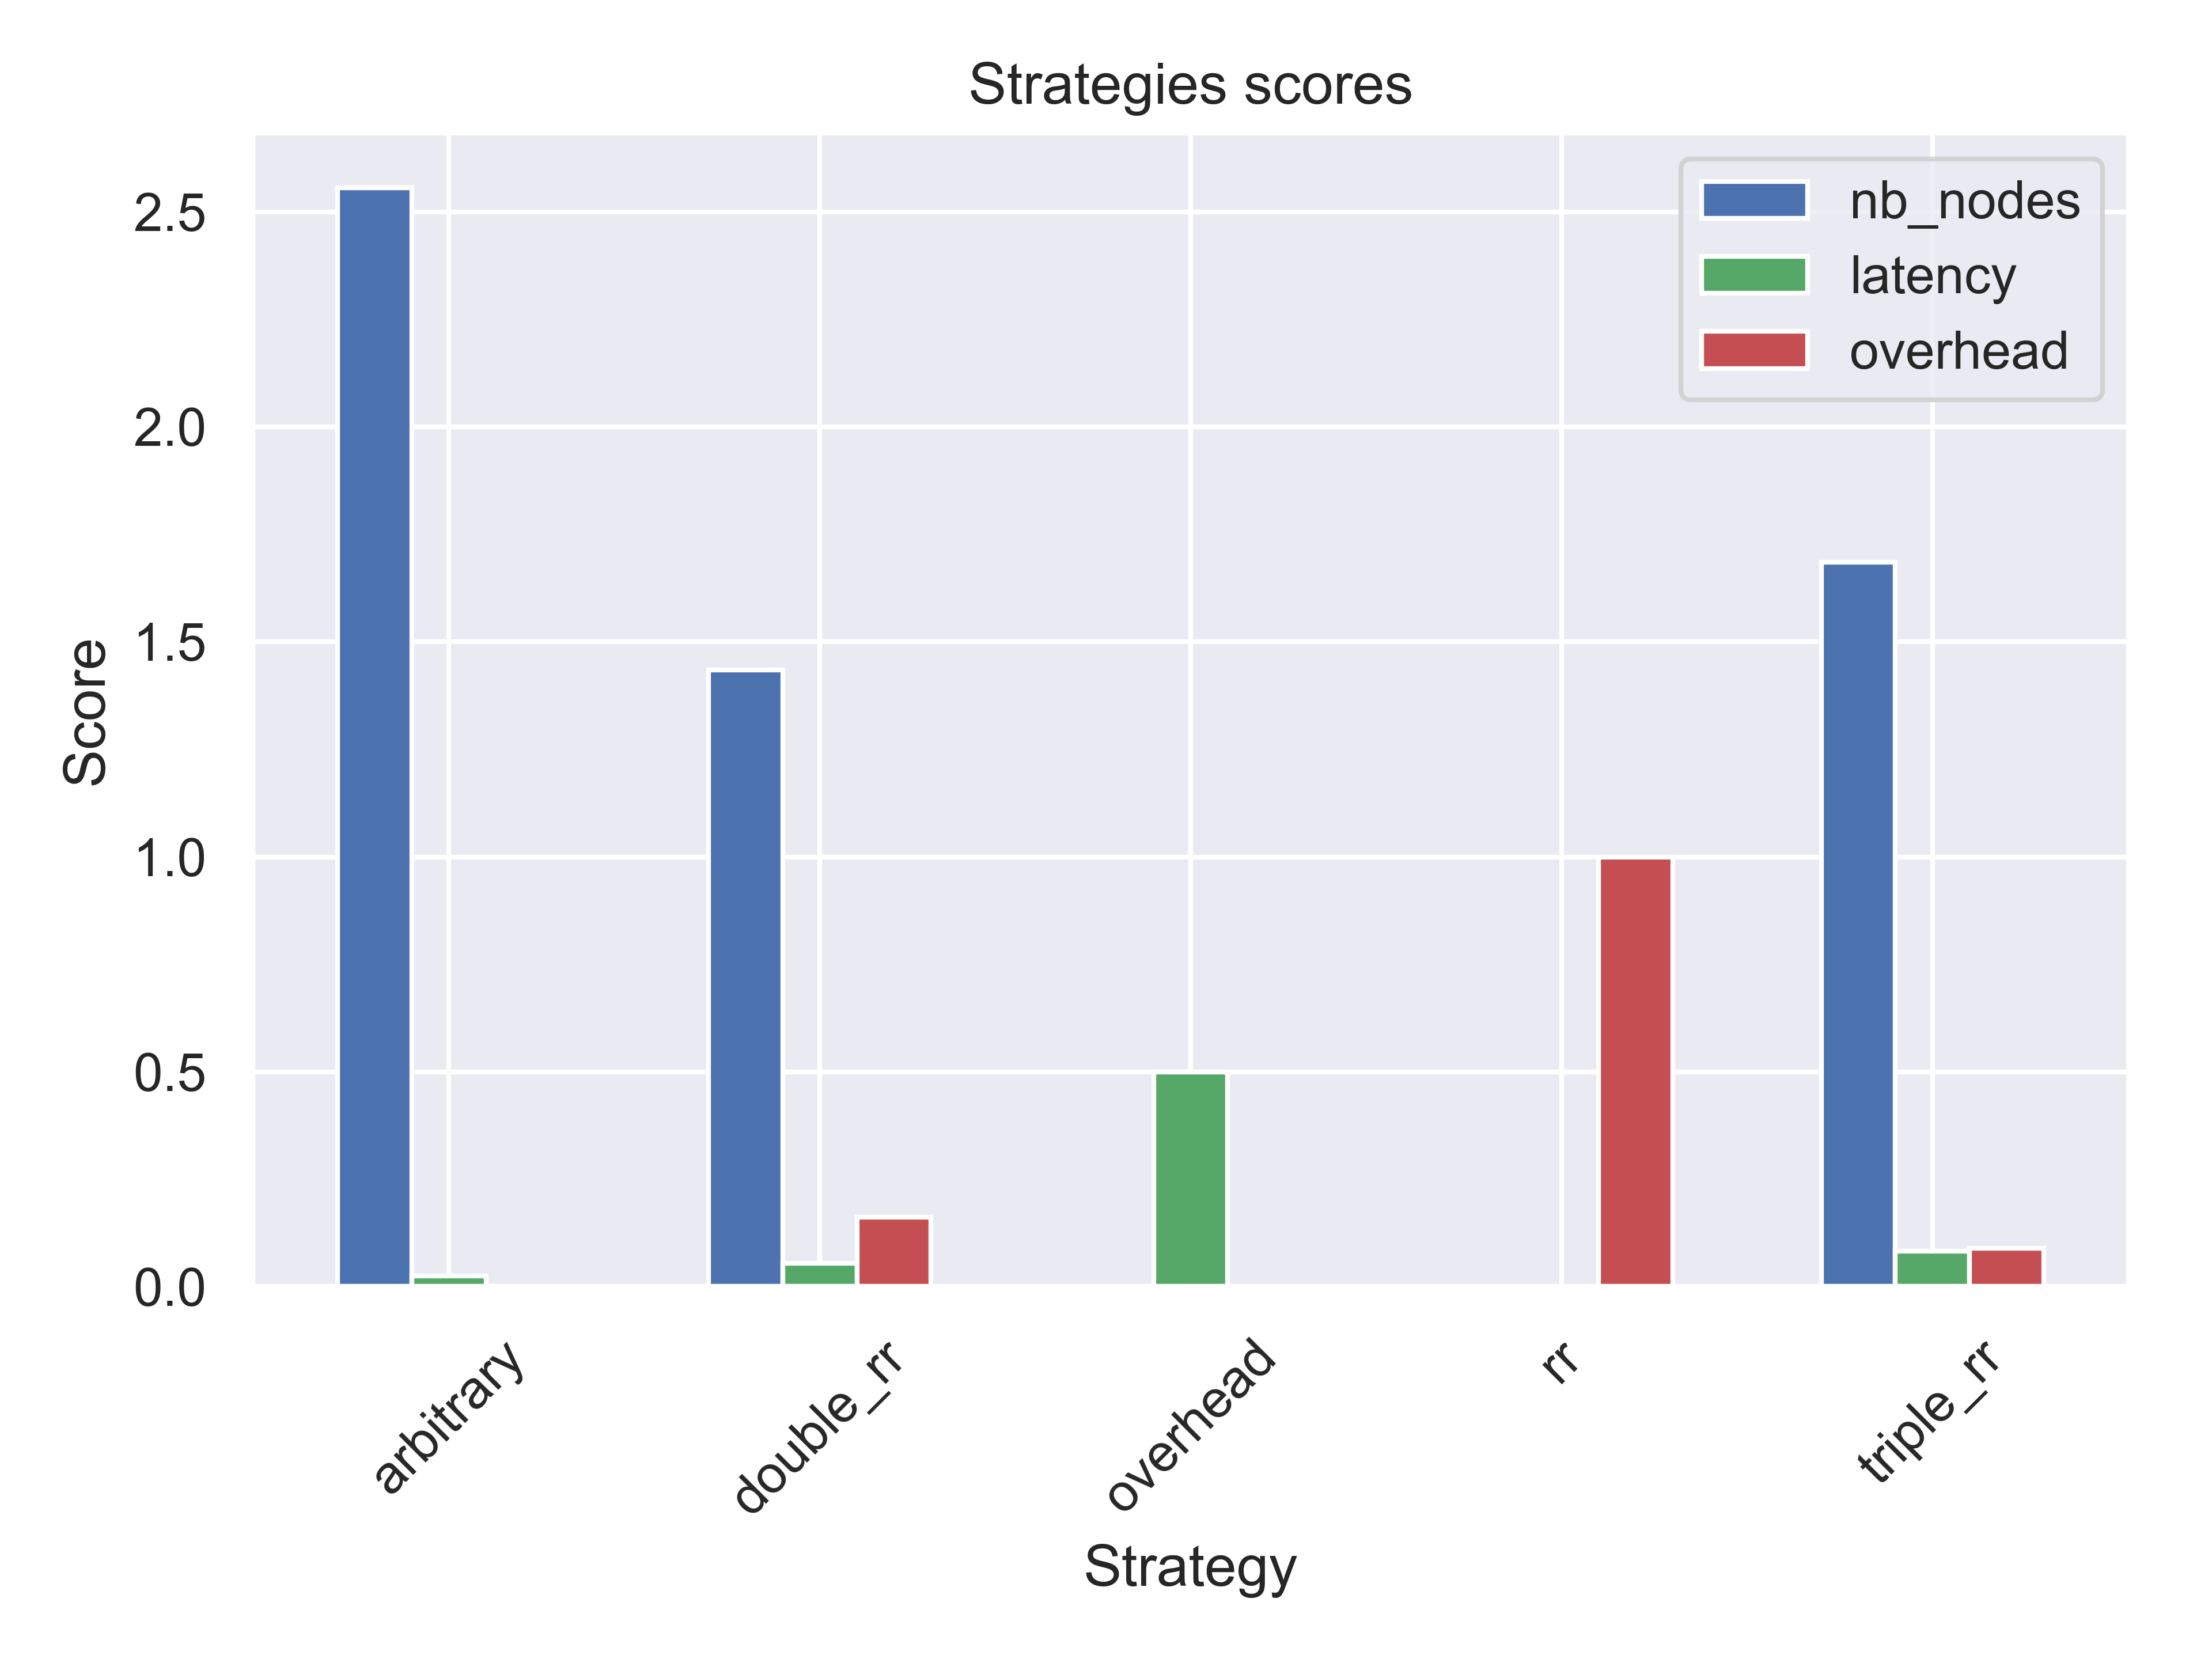
\includegraphics[width=0.8\columnwidth]{final_plot_basic_model}
    \captionsetup{justification=centering}
    \caption{Raw fitted values for the simple model. The strategies are listed
    on the x-axis and their scores are plotted along the y-axis. \todo{prettify
    the x-axis and bar legend}}
    \label{fig:recapTestsPlot}
\end{figure}

\begin{figure}[H]
    \centering
    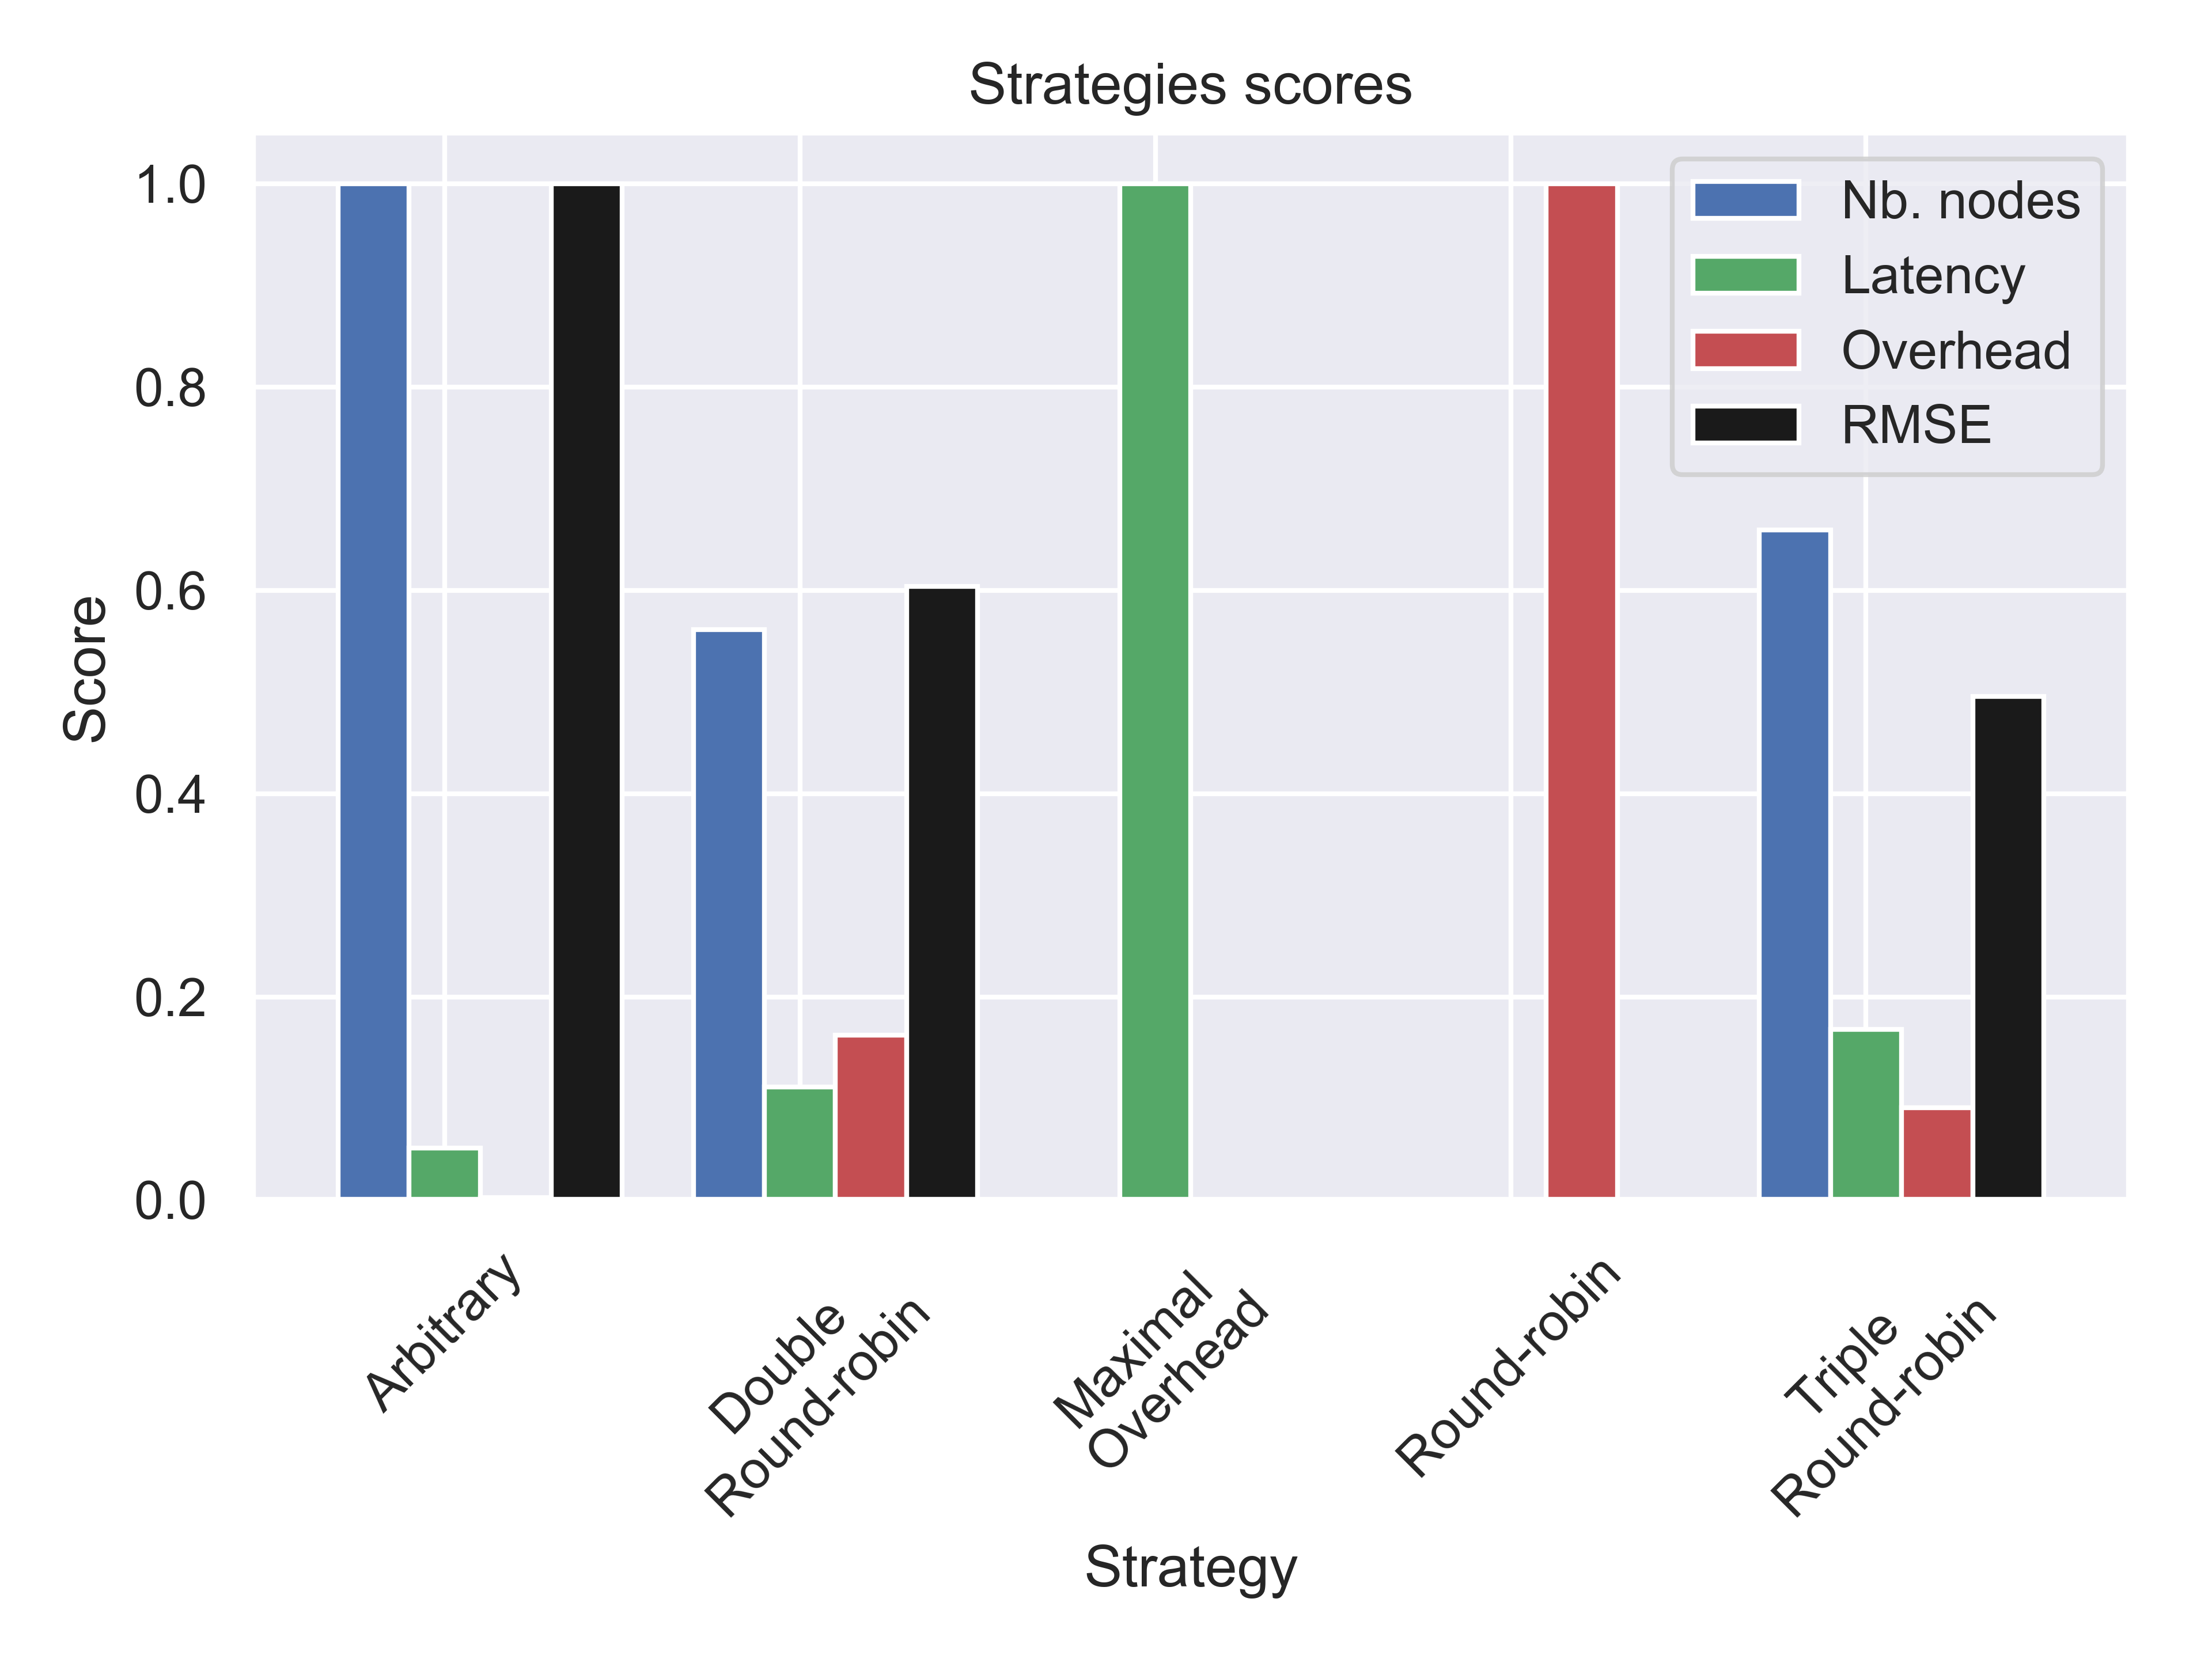
\includegraphics[width=0.8\columnwidth]{final_plot_norm_model}
    \captionsetup{justification=centering}
    \caption{Normalized fitted values for the simple model. The strategies are listed
    on the x-axis and their scores are plotted along the y-axis. \todo{prettify
    the x-axis and bar legend}}
    \label{fig:recapTestsPlot}
\end{figure}


%\begin{table}[H]
%    \centering{
%        \begin{tabular}{|c|c|c|c|}
%            \hline
%            Sending Strategy & \(s_n\) & \(s_l\) & \(s_o\) \\
%            \hline
%            Round-robin & 0.0 & 0.0 &
%            1.0\\
%            \hline
%            Double round-robin & 0.119 & 0.036 & 0.601\\
%            \hline
%            Triple round-robin & 0.404 & 0.082 & 0.401\\
%            \hline
%            Maximal overhead & 0.0 & 0.987 & 0.0\\
%            \hline
%            Arbitrary & 0.861 & 0.035 & 0.106\\
%            \hline
%        \end{tabular}
%        \captionsetup{justification=centering}
%        \caption{Raw fitted values for the simple model, rounded to the 3rd decimal}
%        \label{fig:recapTests}
%    }
%\end{table}

%\begin{figure}[H] 
%    \centering
%    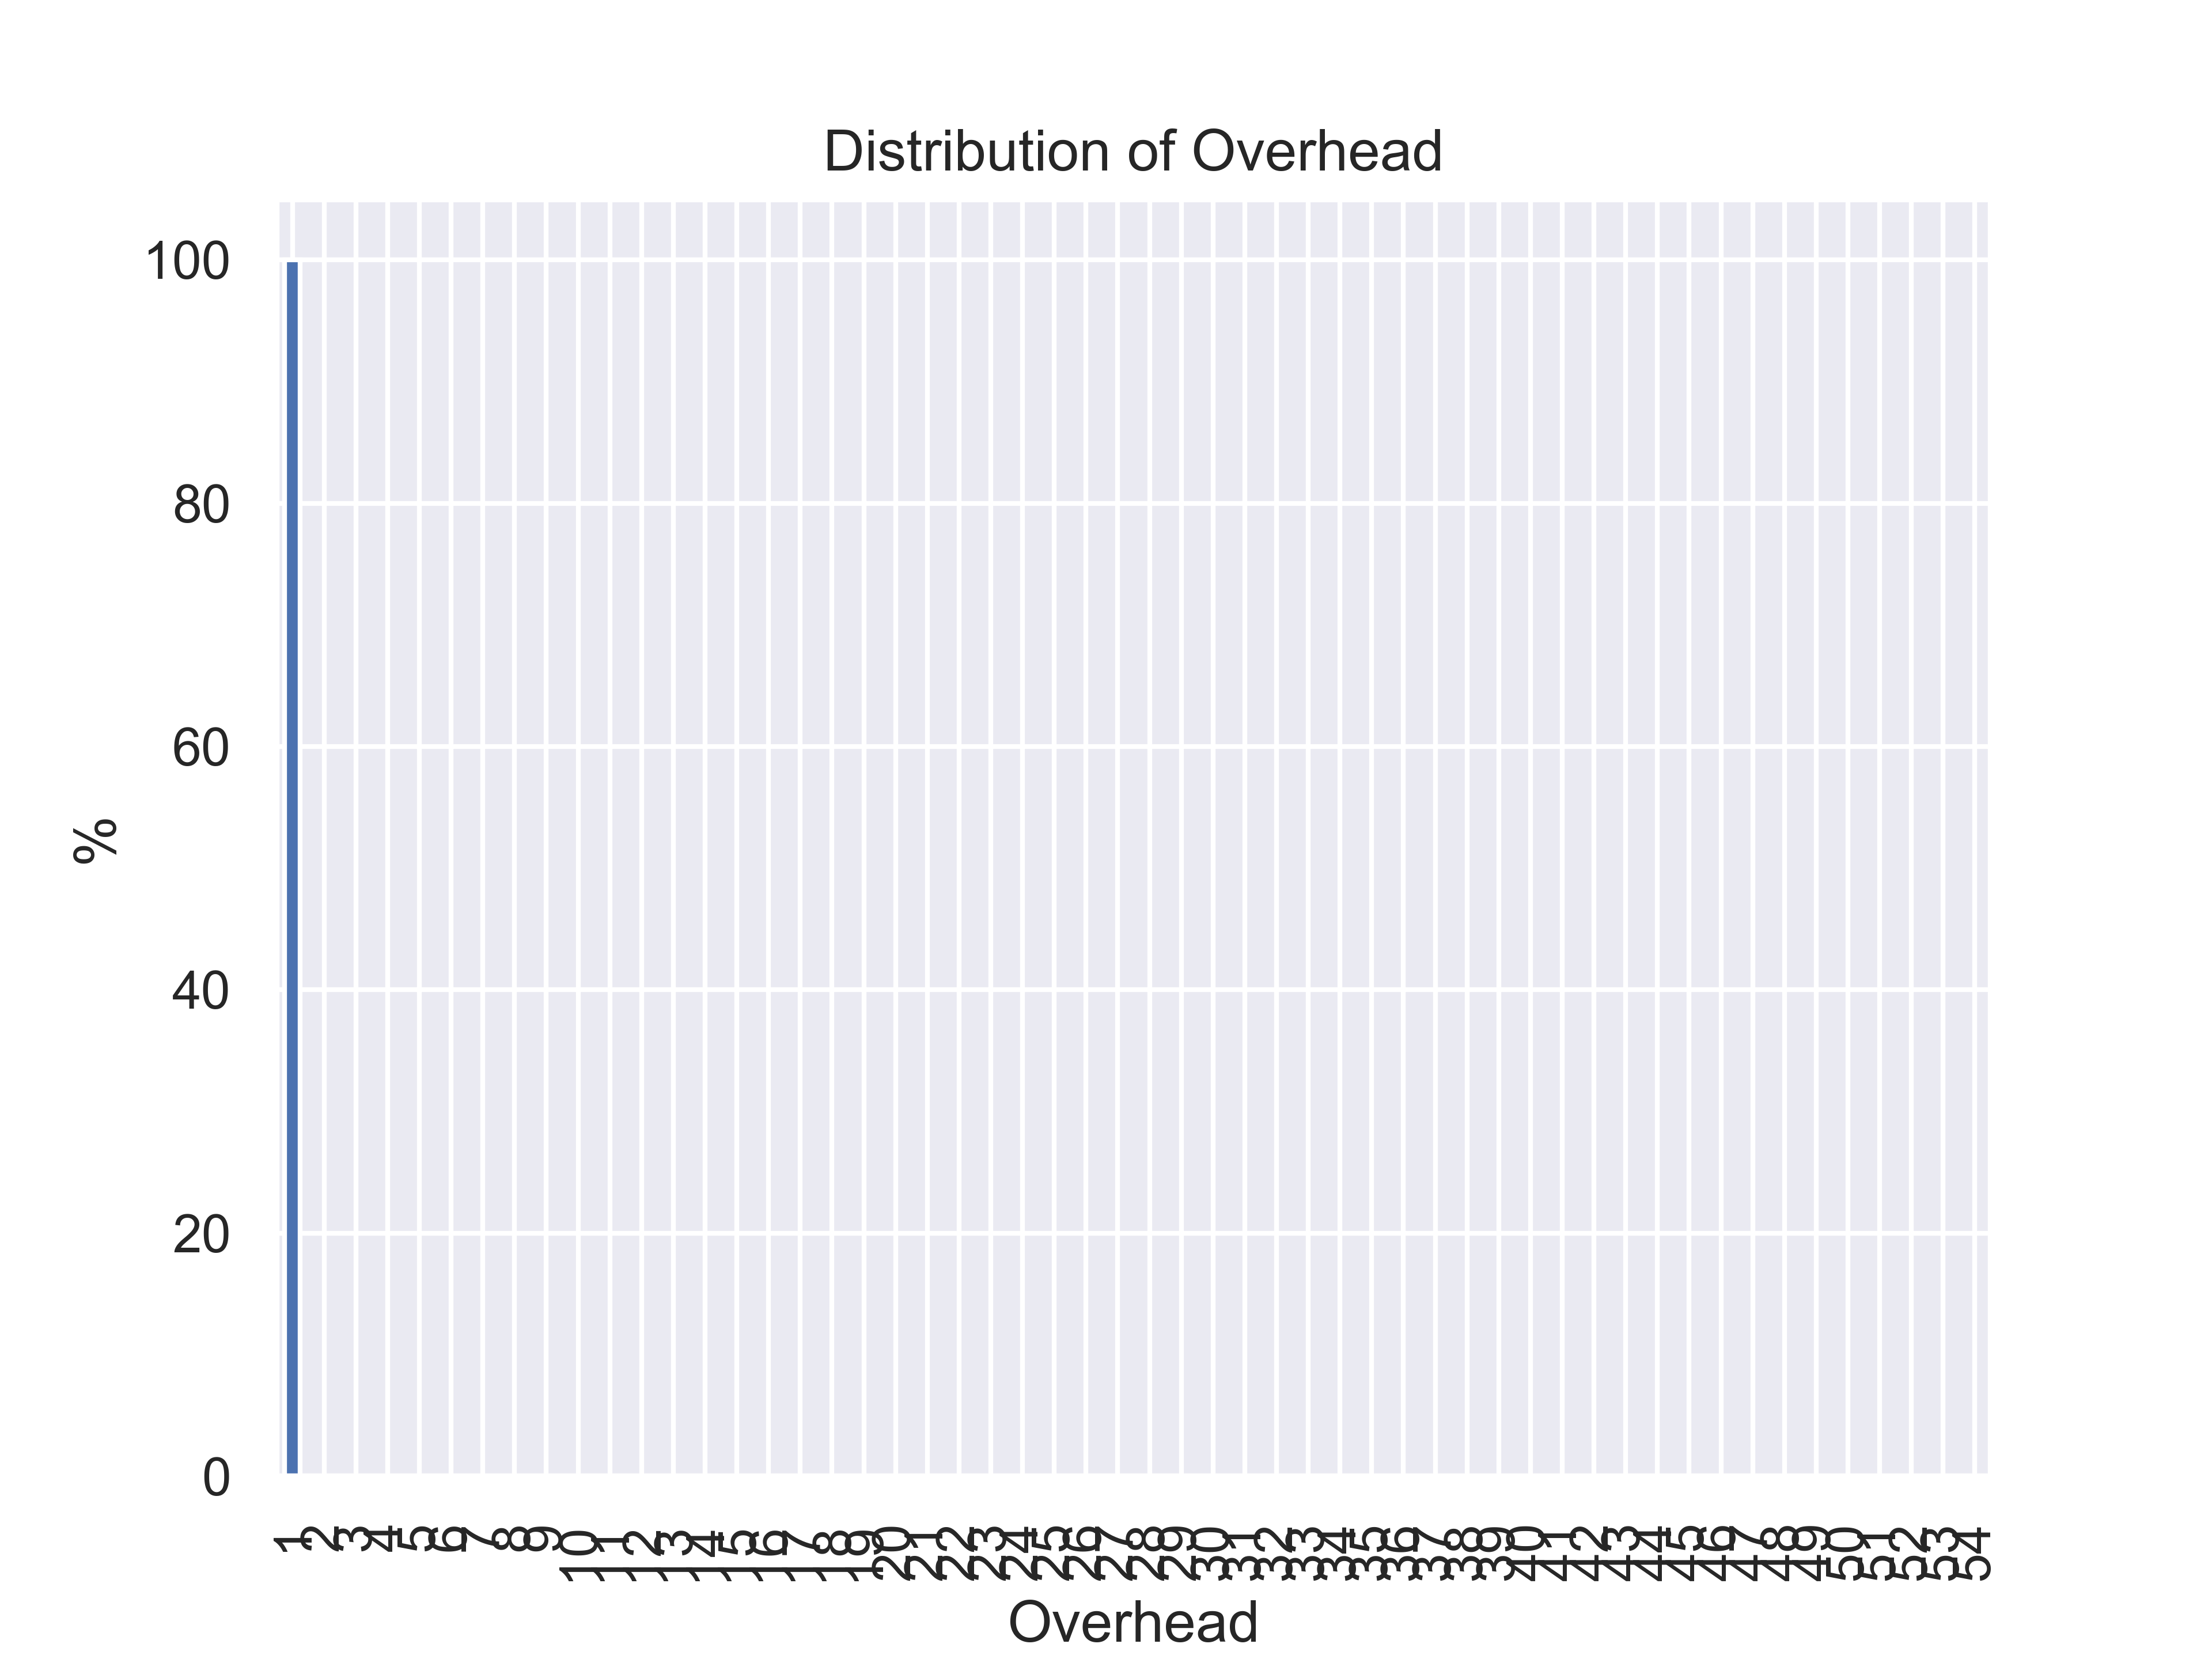
\includegraphics[width=0.8\columnwidth]{hist_overhead_rr_20_nodes_4_depth_all_receivers_gen_averages}
%    \captionsetup{justification=centering}
%    \caption{Histogram of the overhead. Round-robin and all receivers strategies}
%    \label{fig:relOverheadLatencyRR}
%\end{figure}



\subsection{Improvements of the basic model and new fitting}
Show normalized output/radar graphs\
Explain why changing exponents could lead to a better model

\begin{figure}[H]
    \centering
    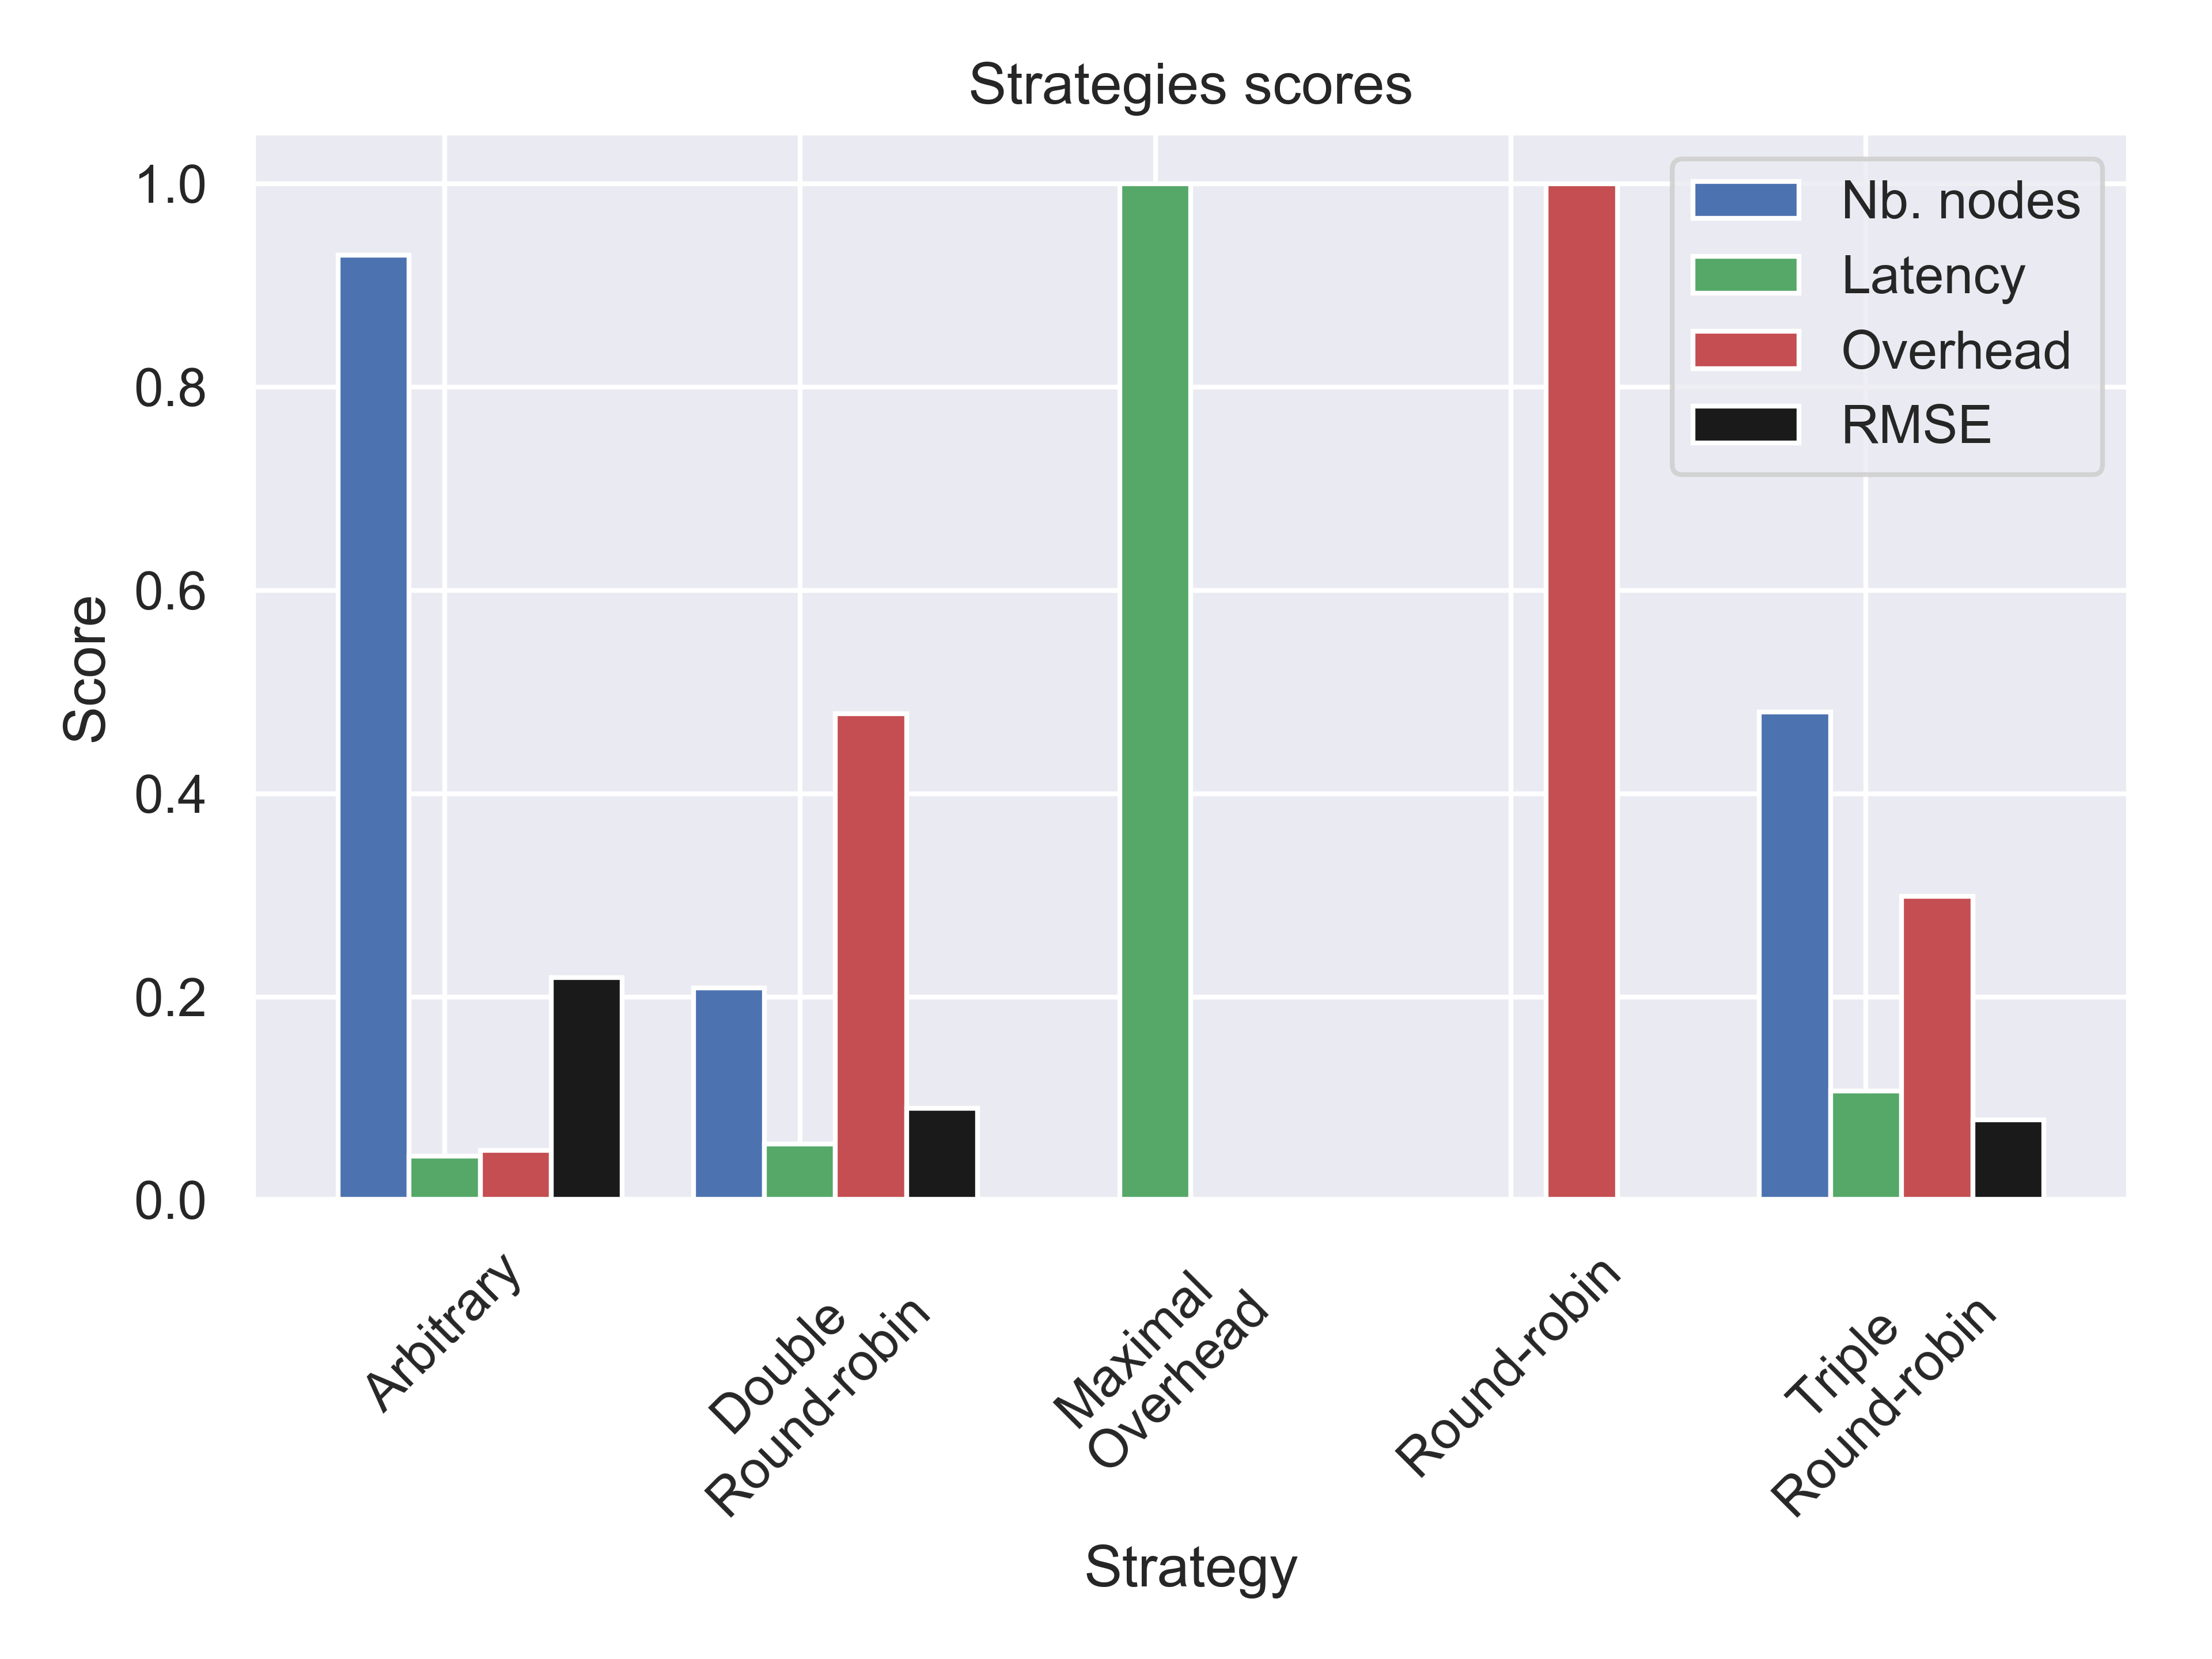
\includegraphics[width=0.8\columnwidth]{final_plot_new_model}
    \captionsetup{justification=centering}
    \caption{Raw fitted values for the improved model. The strategies are listed
    on the x-axis and their scores are plotted along the y-axis. \todo{prettify
    the x-axis and bar legend}}
    \label{fig:recapTestsPlot}
\end{figure}
\section{Analysis}
\todo{why the model is bad according to the number of nodes}

\todo{here will be a table containing all the fitted lines values and a
comparison and explanation of the behaviors that are observed}

\section{Further research}
\subsection{Half set strategy}
A new sending strategy that could be interesting to implement is a strategy
where half the validator set sends a message at each step. That would give a new
comparison point with a fixed latency and an overhead that would be half the one
for the Maximal overhead strategy. It would be useful to have it to find better
coefficients for the refined model.

\subsection{Bottom up strategies}
Now that the framework is functional and can give some reference points and has
ways to compare strategies, one obvious next step would be to implement bottom
up strategies (see \ssec{ssec:bottomUpStrats}) that could include rewarding/slashing the stake of the nodes.

\subsection{Optimize and simplify model}
As seen in the final comparison plots \todo{section}, the model might be too restrictive for
the actual problem. It might be worth trying to find a better fitting model to
better reproduce the real life use case.\
One could argue that tying the number of nodes to the rest of the variables
might be too restrictive, and getting rid of the parameter could offer other
insights while comparing strategies.

\subsection{Better network modeling}
Currently, the \texttt{proptest} implementation does not include a good model
for the network layer. The three proposed receiving strategies are naive but
permitted to validate the framework, from the metrics measurements to the actual
model fitting. A step forward would be to create better models for the
network, based on real life network topologies, latencies, number of nodes, \ldots

